
\chapter{Análise de dados}\label{cap:aplicacao}

%=====================================================

Este capítulo é destinado à análise de dados reais fazendo uso do McGLM e dos testes de hipóteses propostos e implementados neste trabalho. O conjunto de dados utilizado diz respeito a um estudo que visa avaliar se o uso de probióticos é capaz de controlar vício e transtorno da compulsão alimentar em pacientes submetidos à cirurgia bariátrica.

%=====================================================

\section{Contexto}

A cirurgia bariátrica é conhecida como o método mais efetivo no tratamento de obesidade severa pois resulta em considerável perda de peso, remissão de comorbidades e melhora da qualidade de vida dos indivíduos \citep{mechanick2020clinical}.

Os transtornos alimentares são considerados doenças psiquiátricas graves, caracterizadas por comportamento alimentar anormal \citep{treasure2020eating}, dentre os quais transtornos comuns são transtorno da compulsão alimentar e vício alimentar.

O transtorno da compulsão alimentar é reconhecido como um transtorno caracterizado pelo consumo de grandes quantidades de alimentos em um curto período de tempo e uma sensação de perda de controle sobre a alimentação durante esses episódios, associada a angústia e arrependimento ao indivíduo \citep{sarmiento2020diagnostic}, \citep{wilfley2016characteristics}.

Já o vício alimentar está associado ao consumo de alimentos que, em geral são altamente palatáveis (densos em energia, ricos em açúcar, gordura e/ou sal), e por este motivo, excessivamente estimulantes para as vias de recompensa do cérebro, que podem promover o desejo incontrolável e insaciável de continuar comendo e desencadear uma série de sintomas \citep{avena2012further, najem2020prevalence}.

Uma nova abordagem que surge para o tratamento de transtornos psiquiátricos é o uso de probióticos e prebióticos como moduladores do eixo microbiota-intestino-cérebro, também conhecidos como psicobióticos \citep{dinan2013psychobiotics, mason2017feeding, misra2019psychobiotics}.

No entanto, ainda faltam estudos que avaliem a influência da suplementação de probióticos em fatores psicológicos ou comportamentais em indivíduos submetidos à cirurgia bariátrica. Portanto, o objetivo deste estudo foi analisar a influência da suplementação de probióticos no transtorno da compulsão alimentar e no vício alimentar em indivíduos submetidos ao Bypass Gástrico em Y de Roux (RYGB).

%=====================================================

\section{Desenho experimental e coleta de dados}

Trata-se de um ensaio clínico randomizado, duplo-cego, controlado por placebo, realizado com pacientes submetidos ao RYGB no período de abril de 2018 a dezembro de 2019. O estudo foi aprovado pelo Comitê de Ética em Pesquisa da Pontifícia Universidade Católica do Paraná (PUCPR) (nº 4.252.808 ) e registrado pelo Registro Brasileiro de Ensaios Clínicos - REBEC (nºRBR-4x3gqp). A pesquisa foi explicada a cada participante antes de sua participação e, daqueles que concordaram, foi obtido o consentimento informado por escrito.

A divisão dos grupos (placebo ou probiótico) foi feita de forma aleatória. Os critérios de inclusão dos indivíduos no estudo foram: adultos (18-59 anos) que fariam RYGB, com índice de massa corporal (IMC) $\geq$ 35 kg/m2 e que não usaram antibióticos antes da cirurgia. 

Foram retirados do estudo pacientes que foram submetidos a outras técnicas cirúrgicas ou reoperação, tiveram complicações pós-cirúrgicas, fizeram antibioticoterapia concomitante ao uso de probiótico/placebo ou não usaram os comprimidos de probiótico/placebo por mais de nove dias consecutivos. 

Ambos os grupos receberam as mesmas orientações alimentares após a cirurgia, foram acompanhados pela mesma equipe cirúrgica (médico, nutricionista e psicólogo) e tiveram o mesmo número de consultas pré-agendadas antes e após a cirurgia, seguindo o protocolo estabelecido pela instituição onde o estudo foi realizado.

No sétimo dia de pós-operatório, os participantes foram orientados a ingerir dois comprimidos mastigáveis/dia de placebo ou comprimido probiótico Flora Vantage, 5 bilhões de Lactobacillus acidophilus NCFM \textregistered Strain e 5 bilhões de Bifidobacterium lactis Bi-07 \textregistered) da Bariatric Advantage (Aliso Viejo, CA, EUA) por 90 dias.

Os indivíduos foram avaliados em 3 momentos. A primeira avaliação (T0) foi realizada aproximadamente 10 dias antes da cirurgia. As avaliações de acompanhamento foram realizadas aproximadamente três meses (T1) e um ano de pós-operatório (T2). Nestes momentos, foram realizadas avaliações clínicas e antropométricas, bem como os questionários autoaplicáveis foram entregues aos participantes a cada encontro.

A avaliação do transtorno da compulsão alimentar foi feita com base na escala de compulsão alimentar (BES), uma das ferramentas mais usadas para medir a compulsão alimentar em pesquisa, com inúmeros trabalhos comprovando sua eficácia, traduzido para o português e validado para indivíduos com obesidade e submetidos a cirurgia bariátrica. 

Trata-se de um questionário em formato de escala likert de 16 itens, elaborado de acordo com o Manual Diagnóstico e Estatístico de Transtornos Mentais (3ª edição) \citep{spitzer1980diagnostic} por \citet{gormally1982assessment}. Os indivíduos foram orientados a selecionar a opção que melhor representasse sua resposta e o escore final foi a soma dos pontos de cada item, este escore varia de 0 a 46.

Para avaliação de vício alimentar foi utilizada a escala de vício alimentar (YFAS), um questionário que busca detectar sintomas de comportamentos alimentares aditivos. O YFAS foi baseado nos critérios de dependência de substâncias do Manual Diagnóstico e Estatístico IV – Revisão de Texto (DSM-IV-TR) \citep{segal2010diagnostic} e endossado para alimentos altamente processados. Este questionário foi desenvolvido por \citet{gearhardt2009preliminary}. O questionário é uma combinação de 25 opções em escala Likert e a opção de avaliação utilizada foi o número de sintomas de vício.

%=====================================================

\section{Conjunto de dados}\label{sec:dataset}

A amostra final é formada por 71 indivíduos, dos quais 33 pertencem ao grupo placebo e 38 ao grupo tratamento. Se todos estes indivíduos fossem avaliados nos 3 momentos definidos no estudo, o conjunto de dados teria 213 observações. Contudo, ao longo do estudo, diversos indivíduos não compareceram às consultas, o que faz com que haja dados faltantes no conjunto de dados. Após tratamento dos dados e exclusão de observações faltantes restaram 184 observações.

É importante notar que trata-se de um problema com duas variáveis resposta: um escore que caracteriza compulsão e o número de sintomas apresentados que caracterizam vício. Além disso, as observações não são independentes, tendo em vista que medidas tomadas em um mesmo indivíduo são correlacionadas. Portanto, trata-se de um problema que técnicas de modelagem tradicionais seriam de difícil aplicação, mas é um cenário ideal para resolução via McGLM. Além disso, testes de hipóteses podem ser de grande valia para avaliar o efeito da interação entre momento e uso do probiótico sobre vício e compulsão alimentar.

Para fins de análise, o escore que caracteriza compulsão e o número de sintomas apresentados que caracterizam vício foram transformados para a escala unitária, considerando que tratam-se de variáveis restritas. O objetivo da análise é avaliar o efeito de momento e grupo nas métricas de vício e compulsão. O conjunto de dados contém as seguintes variáveis:

\begin{itemize}
  \item id: variável identificadora de indivíduo.
  \item momento: variável identificadora de momento (T0, T1, T2).
  \item grupo: variável identificadora de grupo (placebo, probiótico).
  \item YFAS: proporção de sintomas que caracterizam vício.
  \item BES: proporção de escore de compulsão.
\end{itemize}

%=====================================================

\section{Análise exploratória}

A análise gráfica apresentada na \autoref{fig:descritiva2} mostra, em (a) e (d) que ambas as variáveis de interesse apresentam considerável assimetria à direita. Os boxplots das métricas em função de grupo apresentados em (b) e (e) mostram sensíveis diferenças entre o grupo placebo e probiótico para ambas as respostas. Já os boxplots das métricas em função dos momentos de avaliação, apresentados em (c) e (f), evidenciam que para ambas as métricas os valores eram mais altos no momento T0, havendo considerável redução no momento T1. Quando comparamos T1 e T2, para YFAS parece que há um leve aumento na última avaliação; já para BES, T1 e T2 não parecem diferir.

\begin{figure}[H]
\centering
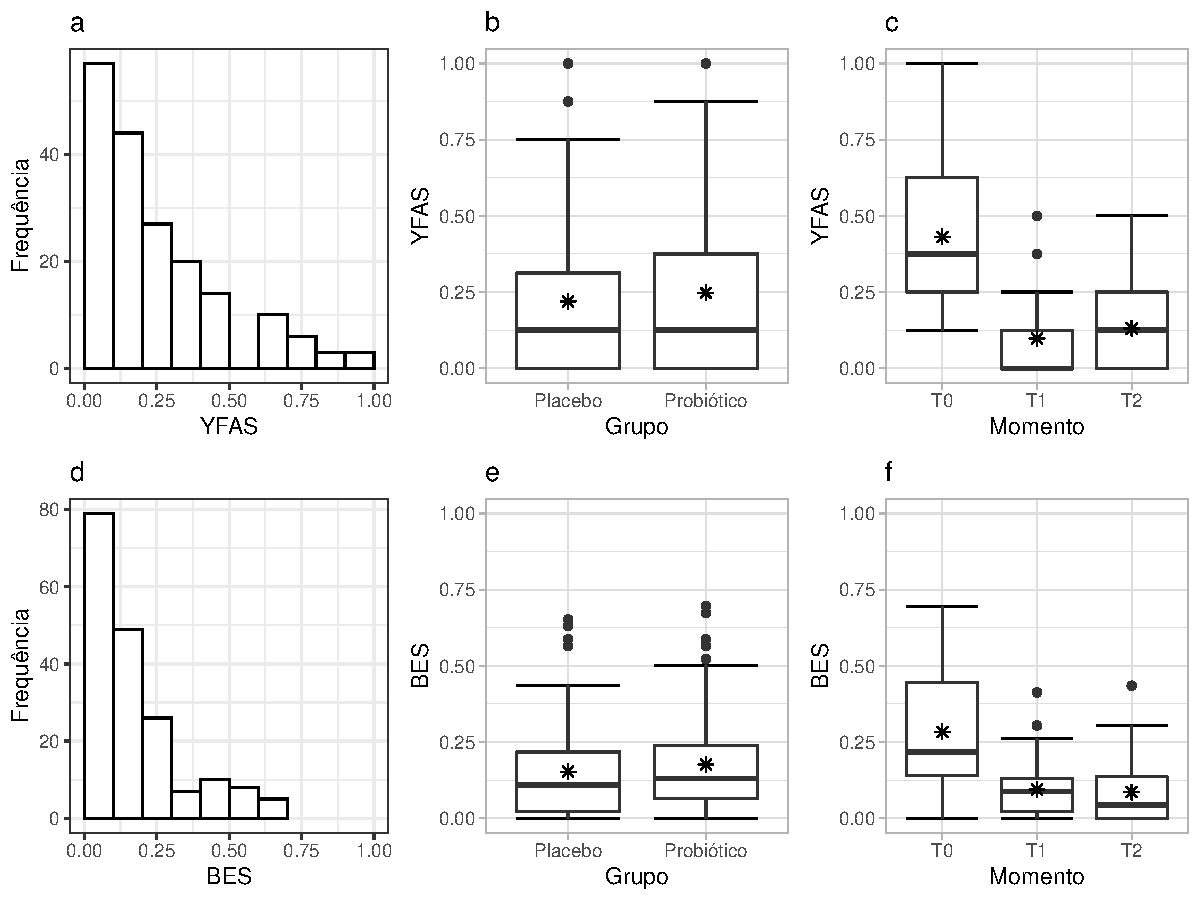
\includegraphics[width=15cm]{/home/lacf14/msc/4_dissertacao/7-aplicacao/descritiva.pdf}
\caption{Análise exploratória gráfica: (a) histograma YFAS, (b) boxplots YFAS em função de grupo, (c) boxplots YFAS em função de momento, (d) histograma BES, (b) boxplots BES em função de grupo, (c) boxplots BES em função de momento. O asterísco nos boxplots indica a média.}
\label{fig:descritiva2}
\end{figure}

Ainda de forma exploratória podemos avaliar o comportamento das métricas de vício e compulsão por meio da avaliação das medidas descritivas por momento e por grupo, apresentadas na \autoref{tab:descritiva1}. É possível verificar a redução de indivíduos ao longo do tempo, algo comum em estudos prospectivos. Quanto às medidas, nota-se que ambos os grupos (placebo ou probiótico) apresentam médias mais altas no momento T0 do que nos demais momentos. Portanto, existe uma clara redução das métricas quando comparado ao pré operatório. Quando comparamos os momentos pós-operatório (T1 e T2) verificamos que as medidas de YFAS, tanto para o grupo placebo quanto para o grupo probiótico apresentam, em média, um aumento das métricas no último momento de avaliação; o mesmo pode ser observado para BES no grupo placebo. Já as medidas de BES no grupo probiótico apresentam queda.

\begin{table}[H]
\centering
\begin{tabular}{ccccc}
\hline
\multirow{2}{*}{Grupo} & \multirow{2}{*}{Momento} & \multirow{2}{*}{n} & YFAS                  & BES                   \\ \cline{4-5} 
                       &                          &                    & Média (desvio padrão) & Média (desvio padrão) \\ \hline
Placebo                & T0                       & 33                 & 0,37 (0,26)           & 0,24 (0,20)           \\
Placebo                & T1                       & 32                 & 0,11 (0,15)           & 0,09 (0,10)           \\
Placebo                & T2                       & 22                 & 0,16 (0,15)           & 0,10 (0,12)           \\
Probiótico             & T0                       & 38                 & 0,49 (0,24)           & 0,32 (0,18)           \\
Probiótico             & T1                       & 37                 & 0,09 (0,12)           & 0,10 (0,08)           \\
Probiótico             & T2                       & 22                 & 0,10 (0,14)           & 0,07 (0,09)           \\ \hline
\end{tabular}
\caption{Número de indivíduos, média e desvio padrão para YFAS e BES para cada combinação de grupo e momento.}
\label{tab:descritiva1}
\end{table}

%=====================================================

\section{Especificação do modelo}

Para análise dos dados foi ajustado um modelo multivariado com os efeitos fixos das variáveis momento e grupo. Adicionalmente, foi incluído no modelo o efeito da interação entre estas duas variáveis explicativas.

Como já mencionado, trata-se de um experimento em que as observações não são independentes pois medidas tomadas em um mesmo indivíduo são correlacionadas e esta correlação deve ser especificada no modelo. 

Como mencionado na \autoref{sec:dataset}, ambas as respostas foram transformadas para a escala unitária, tendo em vista que se tratam originalmente de números inteiros restritos ao intervalo. Por este motivo foi utilizada a função de ligação logito com função de variância binomial. Adicionalmente, estimou-se o parâmetro de potência para todas as respostas em análise. Os preditores lineares são dados por

$$
g_{r}(\mu_{r}) = \beta_{0r} + \beta_{1r} T1 + \beta_{2r} T2 + \beta_{3r} Probiotico + \\ \beta_{4r} T1*Probiotico + \beta_{5r} T2*Probiotico,
$$

\noindent em que o índice $r$ refere-se às variáveis respostas do estudo (1 para YFAS, 2 para BES). Foram consideradas categorias de referência o grupo placebo e o momento T0. $\beta_{0r}$ representa o intercepto, $\beta_{1r}$ o efeito do momento T1, $\beta_{2r}$ o efeito do momento T2, $\beta_{3r}$ o efeito de probiótico. Os parâmetros $\beta_{4r}$ e $\beta_{5r}$ referem-se à interação entre momento e grupo, de tal forma que $\beta_{4r}$ representa o efeito da interação entre T1 e probiótico, e $\beta_{5r}$ representa o efeito da interação entre T2 e probiótico.

Os preditores matriciais, iguais para ambas as respostas, são dados por $h\left \{ \boldsymbol{\Omega}(\boldsymbol{\tau}) \right \} = \tau_0Z_0 + \tau_1Z_1$. A função $h(.)$ utilizada foi a identidade, $\tau_0$ e $\tau_1$ representam os parâmetros de dispersão, $Z_0$ representa uma matriz identidade de ordem, $184 \times 184$ e $Z_1$ representa uma matriz de dimensão $184 \times 184$ especificada de forma a explicitar que as medidas provenientes do mesmo indivíduo são correlacionadas. 

Para exemplificar a forma do preditor matricial, vamos considerar 3 indivíduos: A, B e C. Suponha que o indivíduo A compareceu às 3 consultas, portanto temos informações deste indivíduo em T0, T1 e T2. O indivíduo B compareceu em T0 e T1. Já o indivíduo C compareceu apenas em T0. Deste modo temos 3 indivíduos e 6 observações. Logo $Z_0$ é uma matriz identidade $6 \times 6$ e $Z_1$ é uma espécie de matriz bloco diagonal em que o tamanho dos blocos varia de acordo com o número de medidas para cada indivíduo. Neste cenário o preditor matricial tem a forma

\begin{equation}
h\left \{ \boldsymbol{\Omega}(\boldsymbol{\tau}) \right \} = 
\tau_0 \begin{bmatrix}
1 & 0 & 0 & 0 & 0 & 0\\ 
0 & 1 & 0 & 0 & 0 & 0\\ 
0 & 0 & 1 & 0 & 0 & 0\\ 
0 & 0 & 0 & 1 & 0 & 0\\ 
0 & 0 & 0 & 0 & 1 & 0\\ 
0 & 0 & 0 & 0 & 0 & 1\\ 
\end{bmatrix} + 
\tau_1 \begin{bmatrix}
1 & 1 & 1 & 0 & 0 & 0\\ 
1 & 1 & 1 & 0 & 0 & 0\\ 
1 & 1 & 1 & 0 & 0 & 0\\ 
0 & 0 & 0 & 1 & 1 & 0\\ 
0 & 0 & 0 & 1 & 1 & 0\\ 
0 & 0 & 0 & 0 & 0 & 1\\ 
\end{bmatrix}.
\end{equation}

%=====================================================

\section{Resultados do ajuste}

Com o propósito de verificar a qualidade do ajuste do modelo, foi feita a análise de resíduos do modelo. A análise mostra que os resíduos de Pearson para YFAS e BES apresentam média 0 e desvio padrão próximo de 1. Na \autoref{fig:diagnostico1} são exibidos os histogramas dos resíduos de Pearson por resposta, a distribuição dos resíduos é aproximadamente simétrica com a maior parte dos dados entre -2 e 2.

Na \autoref{fig:diagnostico2} são exibidos os resíduos versos preditos do modelo. Os resultados mostram que não parece haver qualquer tipo de relação entre resíduos e preditos. De forma geral, o modelo parece estar razoavelmente bem ajustado aos dados.

\begin{figure}[H]
\centering
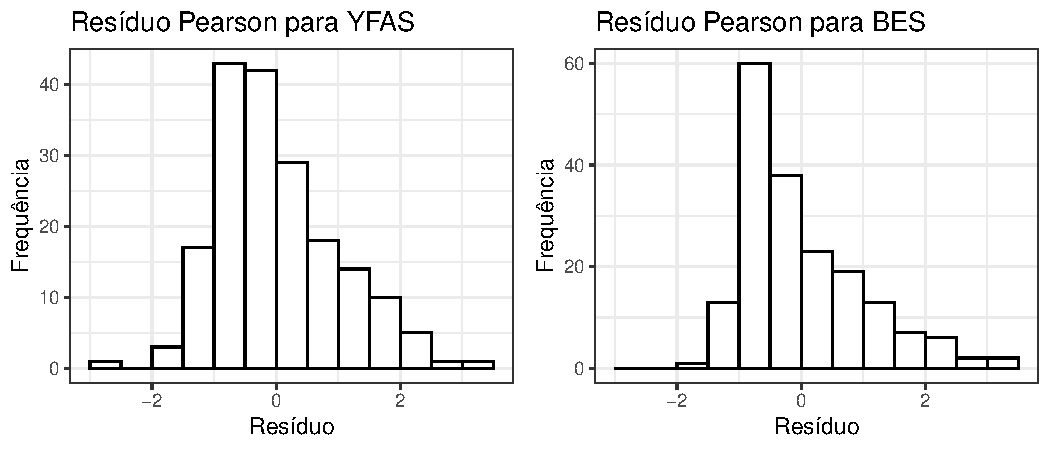
\includegraphics[width=15cm]{/home/lacf14/msc/4_dissertacao/7-aplicacao/res_hist.pdf}
\caption{Histograma dos resíduos de Pearson por resposta.}
\label{fig:diagnostico1}
\end{figure}

\begin{figure}[H]
\centering
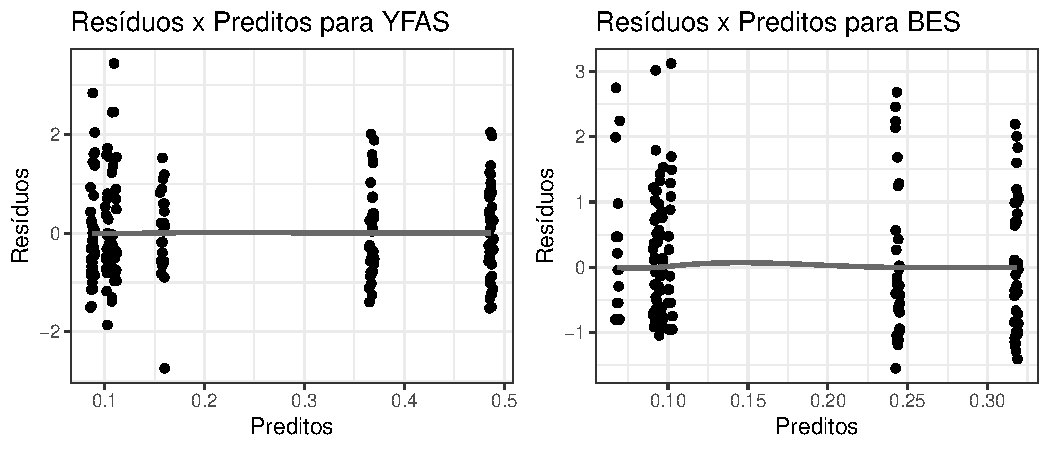
\includegraphics[width=15cm]{/home/lacf14/msc/4_dissertacao/7-aplicacao/res_pred.pdf}
\caption{Gráfico de resíduos Pearson versus preditos com linha de tendência suave para cada resposta.}
\label{fig:diagnostico2}
\end{figure}

As estimativas dos parâmetros, intervalos de confiança assintóticos com 95\% de confiança e valores-p da hipótese de nulidade dos parâmetros são mostrados na \autoref{tab:estimativas}. Adicionalmente, a \autoref{fig:preds} mostra os valores preditos para cada combinação dos fatores para uma melhor interpretação dos resultados.

% Please add the following required packages to your document preamble:
% \usepackage{multirow}
\begin{table}[H]
\centering
\begin{tabular}{c|cccccc}
\hline
\multirow{2}{*}{Parâmetro} & \multicolumn{3}{c}{YFAS}                                                                                             & \multicolumn{3}{c}{BES}                                                                         \\ \cline{2-7} 
                           & Estimativa & \begin{tabular}[c]{@{}c@{}}Intervalo de \\ confiança\end{tabular} & \multicolumn{1}{c|}{Valor-p}        & Estimativa & \begin{tabular}[c]{@{}c@{}}Intervalo de \\ confiança\end{tabular} & Valor-p        \\ \hline
$\beta_0$                  & -0,54      & (-0,87;-0,22)                                                     & \multicolumn{1}{c|}{\textless 0,01} & -1,13      & (-1,44;-0,83)                                                     & \textless 0,01 \\
$\beta_1$                  & -1,55      & (-2,17;-0,94)                                                     & \multicolumn{1}{c|}{\textless 0,01} & -1,16      & (-1,62;-0,69)                                                     & \textless 0,01 \\
$\beta_2$                  & -1,13      & (-1,75;-0,51)                                                     & \multicolumn{1}{c|}{\textless 0,01} & -1,05      & (-1,58;-0,52)                                                     & \textless 0,01 \\
$\beta_3$                  & 0,49       & (0,05;0,93)                                                       & \multicolumn{1}{c|}{0,0284} & 0,37       & (-0,03;0,77)                                                      & 0,0733           \\
$\beta_4$                  & -0,73      & (-1,60;0,14)                                                      & \multicolumn{1}{c|}{0,0}            & -0,33      & (-0,96;0,30)                                                      & 0,3081           \\
$\beta_5$                  & -0,98      & (-1,93;-0,03)                                                     & \multicolumn{1}{c|}{0,0429} & -0,80      & (-1,58;-0,02)                                                     & 0,0449 \\
$\tau_0$                   & 0,18       & (0,01;0,35)                                                       & \multicolumn{1}{c|}{0,0411} & 0,17       & (0,00;0,34)                                                       & 0,0458           \\
$\tau1$                    & 0,01       & (-0,02;0,04)                                                      & \multicolumn{1}{c|}{0,5718}           & 0,04       & (-0,01;0,10)                                                      & 0,1357           \\
$p$                        & 0,91       & (0,47;1,34)                                                       & \multicolumn{1}{c|}{\textless 0,05} & 1,23       & (0,77;1,68)                                                       & \textless 0,05 \\ \hline
\end{tabular}
\caption{Estimativas dos parâmetros, intervalos com 95\% de confiança e valores-p do modelo.}
\label{tab:estimativas}
\end{table}

\begin{figure}[H]
\centering
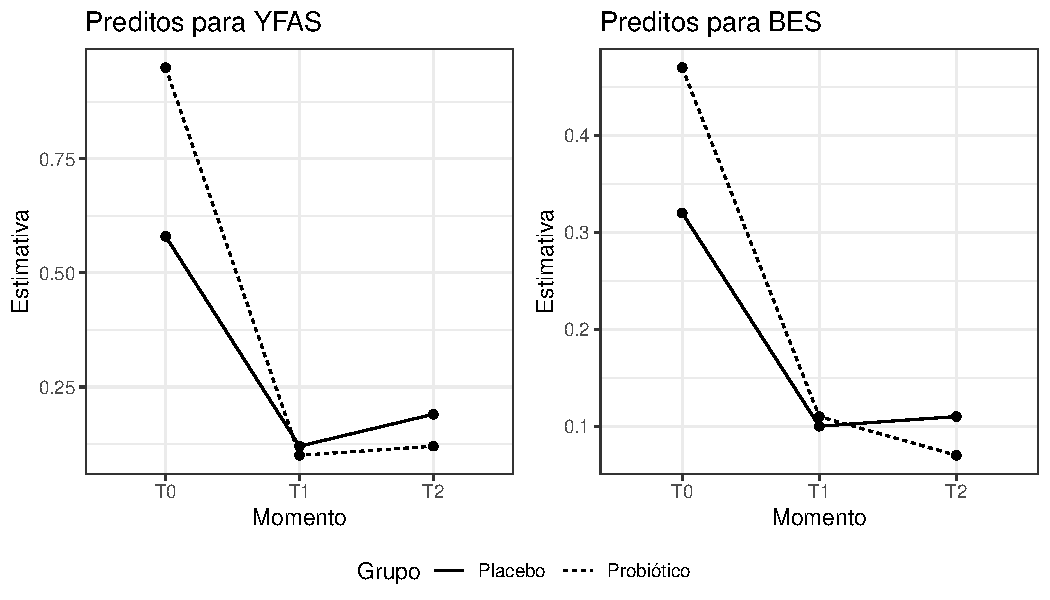
\includegraphics[width=15cm]{/home/lacf14/msc/4_dissertacao/7-aplicacao/fig_preditos.pdf}
\caption{Gráfico de preditos pelo modelo para cada combinação entre momento e grupo.}
\label{fig:preds}
\end{figure}

%=====================================================

\section{Testes de hipóteses}

Até este ponto foi apresentada uma análise padrão, com os resultados usuais da análise de um modelo de regressão. Indo mais além nesta análise, podemos fazer uso dos resultados e implementações deste trabalho.

Podemos optar por uma análise de variância multivariada do tipo II para avaliar a importância das variáveis no problema. O resultado, apresentado na tabela \autoref{tab:manovaII} aponta para existência significativa do efeito de momento e ausência de efeito de grupo, indicando que para ambas as respostas as métricas se alteram ao longo do tempo mas sem alteração entre grupos.

\begin{table}[H]
\centering
\begin{tabular}{cccc}
\hline
Variável      & Graus de liberdade & Qui-quadrado & Valor-p        \\ \hline
Intercepto    & 2                  & 53,1581      & \textless 0,01 \\
Momento       & 8                  & 139,0161     & \textless 0,01 \\
Grupo         & 6                  & 8,4928       & 0,2042         \\
Momento*Grupo & 4                  & 6,9923       & 0,1363         \\ \hline
\end{tabular}
\caption{Análise de variância multivariada tipo II.}
\label{tab:manovaII}
\end{table}

A fim de avaliar os resultados por resposta, podemos utilizar uma análise de variância univariada do tipo II. Os resultados são apresentados na \autoref{tab:anovaII}. Considerando um nível de significância de $0,01$, existe evidência que aponta para efeito de momento.

\begin{table}[H]
\centering
\begin{tabular}{c|c|cc|cc}
\hline
              &                    & \multicolumn{2}{c|}{YFAS}     & \multicolumn{2}{c}{BES}       \\ \hline
Variável      & Graus de liberdade & Qui-quadrado & Valor-p        & Qui-quadrado & Valor-p        \\ \hline
Intercepto    & 1                  & 10,6128      & \textless 0,01 & 53,1473      & \textless 0,01 \\
Momento       & 4                  & 102,9875     & \textless 0,01 & 99,5681      & \textless 0,01 \\
Grupo         & 3                  & 6,6837       & 0,0827         & 5,3083       & 0,1506         \\
Momento*Grupo & 2                  & 5,5984       & 0,0609         & 4,2477       & 0,1196         \\ \hline
\end{tabular}
\caption{Análise de variância univariada do tipo II.}
\label{tab:anovaII}
\end{table}

Como as análises de variâncias apontaram para efeito significativo de variáveis categóricas, podemos explorar quais níveis diferem entre si. A \autoref{tab:mul-multcomp1} apresenta as comparações duas a duas entre momentos. Os resultados mostram que, para ambas as respostas existem diferenças entre o primeiro versus segundo e primeiro versus terceiro momento, mas os dois últimos momentos não diferem entre si.

\begin{table}[H]
\centering
\begin{tabular}{cccc}
\hline
Contraste & Graus de liberdade & Qui-quadrado & Valor-p        \\ \hline
T0-T1     & 2                  & 97,9874      & \textless 0,01 \\
T0-T2     & 2                  & 67,2462      & \textless 0,01 \\
T1-T2     & 2                  & 2,4730       & 0,8712         \\ \hline
\end{tabular}
\caption{Comparações duas a duas entre momentos para ambas as respostas.}
\label{tab:mul-multcomp1}
\end{table}

A tabela \autoref{tab:mul-multcomp3} apresenta as comparações entre grupos para cada momento para ambas as respostas. Os resultados apontam para a ausência de diferença entre grupos em cada momento.

\begin{table}[H]
\centering
\begin{tabular}{cccc}
\hline
Contraste                & Graus de liberdade & Qui-quadrado & Valor-p \\ \hline
T0:Placebo-T0:Probiótico & 2                  & 5,5819       & 0,9204  \\
T1:Placebo-T1:Probiótico & 2                  & 0,6096       & 1       \\
T2:Placebo-T2:Probiótico & 2                  & 1,7645       & 1       \\ \hline
\end{tabular}
\caption{Comparações duas a duas entre grupos para cada momento para ambas as respostas.}
\label{tab:mul-multcomp3}
\end{table}

No modelo, incluímos a informação de que existem medidas que foram tomadas em um mesmo indivíduo. Esta informação é declarada no preditor matricial que estima um parâmetro de dispersão associado à matriz que aponta a relação entre os indivíduos. Uma hipótese de interesse pode ser avaliar se existe evidência para crer que, neste problema, as medidas tomadas em um mesmo indivíduo são de fato correlacionadas. Para isso podemos postular hipóteses sobre os parâmetros de dispersão. Tal como nas análises de variância, isso pode ser feito por resposta ou para ambas as respostas simultaneamente.

A \autoref{tab:manova_disp} apresenta os resultados do teste multivariado, ou seja, avalia a hipótese de que em ambas as respostas as medidas sejam correlacionadas. Os resultados apontam que não há evidência para crer que as medidas tomadas em um mesmo indivíduo apresentam correlação.

\begin{table}[H]
\centering
\begin{tabular}{cccc}
\hline
Variável               & Graus de liberdade & Qui-quadrado & Valor-p        \\ \hline
$\tau_0$ & 2                  & 7,1936       & 0,0274 \\
$\tau_1$ & 2                  & 2,3201       & 0,3135         \\ \hline
\end{tabular}
\caption{Análise de variância multivariada do tipo III para parâmetros de dispersão.}
\label{tab:manova_disp}
\end{table}

%=====================================================

Com isso, apresentamos uma análise de dados real, em que o uso de testes de hipóteses para avaliação de parâmetros de um modelo multivariado se mostrou de grande valia para extrair o máximo de informações a respeito do problema. Exploramos testes sobre parâmetros de regressão e dispersão a fim de concluir investigar os elementos associados ao desfecho dos fenômenos sob análise.
